UI is the graphic feature of the application mainly responsible for the displaying information and interact with the user. UI consist of login subsystem responsible for taking userid and password from user. Registration subsystem is responsible to take userid, email, password, full name from the user. Add\_Shelf subsystem is responsible for taking the shelf description from the user. Add\_Item is responsible for taking item description from user. Search subsystem is responsible for taking user input via QR code or input text. After any kind input and options chosen by the user UI\_Controller will send all user input and the option chosen by the user to Business\_Controller in Business\_Logic. UI\_Controller also accept the input messages from the Business\_Controller, stating successful completion of the chosen task by the user.

\subsection{Layer Hardware}
Being an android/IOS application, our UI will use underlying hardware for user input and to display information to the users. i.e input are done by using phones screen and output are shown in same screen. 
\subsection{Layer Operating System}
IOS/Andriod

\subsection{Layer Software Dependencies}
Our application uses React native as a framework for all UI layer and 

\subsection{Subsystem 1}
Descibe at a high level the purpose and basic design of this subsystem. Is it a piece of hardware, a class, a web service, or something else? Note that each of the subsystem items below are meant to be specific to that subystem and not a repeat of anything discussed above for the overall layer.

\begin{figure}[h!]
	\centering
 	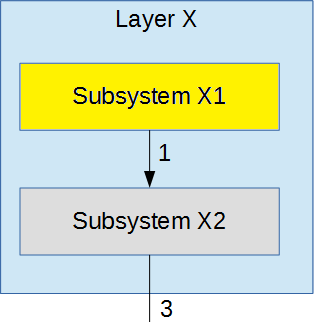
\includegraphics[width=0.60\textwidth]{images/subsystem}
 \caption{Example subsystem description diagram}
\end{figure}

\subsubsection{Subsystem Hardware}
A description of any involved hardware components for the subsystem.

\subsubsection{Subsystem Operating System}
A description of any operating systems required by the subsystem.

\subsubsection{Subsystem Software Dependencies}
A description of any software dependencies (libraries, frameworks, design software for mechanical parts or circuits, etc) required by the subsystem.

\subsubsection{Subsystem Programming Languages}
A description of any programming languages used by the subsystem.

\subsubsection{Subsystem Data Structures}
A description of any classes or other data structures that are worth discussing for the subsystem. For example, data being transmitted from a microcontroller to a PC via USB should be first be assembled into packets. What is the structure of the packets?

\subsubsection{Subsystem Data Processing}
A description of any algorithms or processing strategies that are worth discussing for the subsystem. If you are implementing a well-known algorithm, list it. If it is something unique to this project, discuss it in greater detail.


